\section{No flavour changing neutral currents at tree level}
\label{sec:tree_fcnc}
The quark mixing that allows now the transition between up and down as well as up and strange does not introduce flavour changing couplings to the $Z$.

For this section we need some math that is beyond the scope of this course (you'll learn about this in the 4th year particle physics course). To follow the rest of this (starred - meaning non examinable) subsection, I need to ask you to accept the following without proof:
\begin{enumerate}[i)]
\item A function called "the Lagrangian" encodes all the physics there is. It is a function of fields. Each type of particle has an associated field. Particles are excitations of these fields.
\item All we need to know for this section is that, whenever there is a term with three particle fields in the Lagrangian, there is a corresponding Feynman rule for a 3-prong vertex (btw, terms with four particle fields give a 4-prong vertex etc). E.g. ABC leads to a vertex like this:
\\
\parbox[c]{0.3\textwidth}{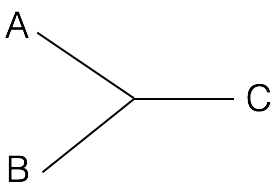
\includegraphics[width=0.3\textwidth]{fig/C_P_CP/ABC_vtx}}
\\
(and also like this:
\parbox[c]{0.2\textwidth}{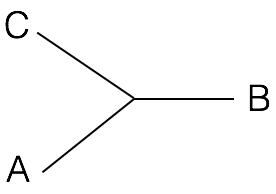
\includegraphics[width=0.2\textwidth]{fig/C_P_CP/CAB_vtx}}
and this:
\parbox[c]{0.2\textwidth}{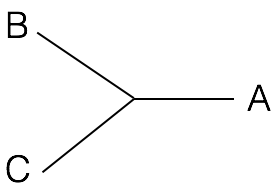
\includegraphics[width=0.2\textwidth]{fig/C_P_CP/BCA_vtx}}.)
\end{enumerate}

 The terms describing the interaction of the down-type quarks with the $Z$ are proportional to $Z\bar{d}d + Z\bar{s}s$. Replacing now $d, s$ with $d', s'$ we get:
\begin{eqnarray}
 Z\bar{d}'d' + Z\bar{s}'s'
&=&
 Z\left(-\bar{s}\sin\theta_C + \cos\theta_C \bar{d}\right)
 \left(-s\sin\theta_C + \cos\theta_C d\right)
\nonumber\\
&&+
 Z\left( \bar{d}\sin\theta_C + \cos\theta_C \bar{s}\right)
 \left( d\sin\theta_C + \cos\theta_C s\right)
\nonumber\\
&=&
  Z\bar{s}s \left(\sin^2\theta_C + \bar{d}d \cos^2\theta_C
- (\bar{s}d + \bar{d}s) \sin\theta_C\cos\theta_C\right)
\nonumber\\
&=&
  Z\left(\bar{d}d \sin^2\theta_C + \bar{s}s \cos^2\theta_C
+ (\bar{s}d + \bar{d}s) \sin\theta_C\cos\theta_C\right)
\nonumber\\
&=& Z\bar{d}d + Z\bar{s}s 
\end{eqnarray}
So the basis change that we did for the down-type quark relative to the up quark does nothing to the $Z$ couplings, they are exactly as before (and forbid flavour changing interactions, i.e. no $d \to s$ transitions) at tree levels.

Note that the notion of an $s'$ quark, which is needed for the FCNC to cancel, only makes sense if there is also another up-type quark, the charm. So this is actually already an aspect of the GIM mechanism, described below.
